\documentclass[a4paper,10pt]{scrartcl}

\usepackage[utf8]{inputenc}
\usepackage[T1]{fontenc}    
\usepackage{fourier,euler}     
\usepackage{amsmath,amsthm,amssymb}
\usepackage{graphicx}

\usepackage[french]{babel}
\usepackage{hyperref}
\usepackage{microtype}    

% THEOREMES/EXERCICES
\theoremstyle{definition}
	\newtheorem{defi}{Définition}[section]
\theoremstyle{remark}
	\newtheorem*{remarque}{Remarque}
	\newtheorem*{exemple}{Exemple}
\theoremstyle{plain}
	\newtheorem{thm}[defi]{Théorème}
	\newtheorem{proposition}[defi]{Proposition}
	\newtheorem{exo}{Exercice}[section]
	\newenvironment{sol}[1]{\noindent\textbf{Correction de l'exercice~\ref{#1}.}\par}{}


% COMMANDES PERSONNELLES
\newcommand{\celsius}{^\circ C}

\newcommand{\ensemble}[1]{\mathbb{#1}}
\newcommand{\R}{\ensemble{R}}

\newcommand{\differential}[1]{\,\mathrm{d}#1}
\newcommand{\dx}{\differential{x}}
\newcommand{\dt}{\differential{t}}
\newcommand{\dT}{\differential{T}}

% TITRE DU DOCUMENT
\title{Équations différentielles}
\author{Votre Nom}
\date{15 janvier 2014}

\begin{document}
\maketitle
\tableofcontents


\section*{Introduction}
Les équations différentielles décrivent l'évolution de nombreux phénomènes dans des domaines variés. Une équation différentielle est une équation impliquant une ou plusieurs dérivées d'une fonction inconnue. Si toutes les dérivées sont prises par rapport à une seule variable, on parle d'équation différentielle ordinaire. Une équation mettant en jeu des dérivées partielles est appelée équation aux dérivées partielles.


\section{Rappels}
Une équation différentielle (EDO) de premier ordre est une équation exprimée sous la forme d'une relation 
\begin{equation}\label{eq.edo}
F(t,y(t),y'(t))=0
\end{equation}
\begin{itemize}
\item dont l'inconnue est une fonction $y\colon I\subset\R\to\R$ définie sur un intervalle $I$ (à déterminer)
\item dans laquelle cohabitent à la fois $y$ et sa dérivée $y'$.
\end{itemize}
\emph{Résoudre une équation différentielle}, c'est chercher toutes les fonctions, définies sur un intervalle $I\subset\R$, qui satisfont l'équation~\eqref{eq.edo}. 

\begin{exemple}
Résoudre l'équation différentielle $y'(t)=-y(t)$ signifie chercher toutes les fonctions
\begin{align*}
y\colon I\subset\R&\to\R\\
t&\mapsto y=f(t)
\end{align*}
telles que $f'(t)=-f(t)$ pour tout $t\in I$. Toutes les solutions s'écrivent $f(t)=ce^{-ct}$ pour tout $t\in\R$ (où $c$ est une constante réelle quelconque).  
\end{exemple}


\subsection{Condition initiale}
Une EDO admet généralement une infinité de solutions. Pour en sélectionner quelques unes on doit imposer une condition supplémentaire qui correspond à la valeur prise par la solution en un point de l'intervalle d'intégration. 
\begin{defi}[Condition initiale]
Une condition initiale (CI) est une relation du type $y(t_0)=y_0$ qui impose en $t_0$ la valeur $y_0$ de la fonction inconnue.
\end{defi}
En pratique, se donner une CI revient à se donner le point $(t_0,y_0)$ par lequel doit passer le graphe de la fonction solution.


\subsection{Problème de \textsc{Cauchy}}
Le couple EDO-CI porte le nom de \flqq problème de \textsc{Cauchy}\frqq:
\begin{defi}[Problème de \textsc{Cauchy}]
Soit $\varphi \colon \R \times \R \to \R$ une fonction donnée et $y'$ la dérivée de $y$ par rapport à $t$. On appelle \emph{problème de \textsc{Cauchy}} le problème
\begin{itemize}
\item[]trouver une fonction $y \colon I\subset \R \to \R$ définie sur un intervalle $I$ telle que
\begin{equation}\label{pbCauchy}
\begin{cases}
y'(t) = \varphi(t,y(t)), &\forall t \in I,\\
y(t_0) = y_0,
\end{cases}
\end{equation}
\end{itemize}
avec $t_0$ un point de $I$ et $y_0$ une valeur donnée.
\end{defi}

Il y a un résultat qui garantit que, sous certaines hypothèses très générales, deux graphes de fonctions qui sont des solutions de la même EDO ne se rencontrent jamais. Le théorème garantit aussi l'existence des solutions; pour donner un énoncé précis, il faut d'abord définir la notion de solution maximale.


\subsubsection{Solution maximale}
De façon générale, lorsqu'on se donne une équation différentielle et une condition initiale $y(t_0) = y_0$, on cherche un intervalle $I$, contenant $t_0$, sur lequel une solution existe, et qui soit \flqq le plus grand possible\frqq: il n'existe pas d'intervalle plus grand sur lequel l'équation différentielle ait une solution. Cet intervalle s'appelle \emph{intervalle de vie} de la solution. Une solution définie sur cet intervalle le plus grand possible s'appelle \emph{solution maximale}.
\begin{defi}[Solution maximale]
On se donne une équation différentielle $y'(t)=\varphi(t,y(t))$ avec une condition initiale $y(t_0)=y_0$. Une \emph{solution maximale} pour ce problème est une fonction $y=f(t)$, définie sur un intervalle $I$ appelé \emph{intervalle de vie}, telle que
\begin{itemize}
\item $f$ est solution de l'équation différentielle et vérifie la condition initiale;
\item il n'existe pas de solution $\tilde f$ de la même équation, vérifiant la même condition initiale et définie sur un intervalle $J$ contenant $I$ et plus grand que $I$.
\end{itemize}
\end{defi}

\begin{proposition}\label{prop.asymptote}
Soit $y=f(t)$ une solution maximale définie sur un intervalle de vie $I=]a;b[$. Si $b\neq+\infty$ alors
\[
\lim_{t\to b-}y(t)=\pm\infty,
\]
autrement dit le graphe de la solution a une asymptote verticale en $t=b$. Même chose si $a\neq-\infty$.
\end{proposition}
On utilise souvent le corollaire~\ref{prop.asymptote} sous forme contraposée: si les solutions ne peuvent pas \flqq exploser\frqq, alors elles sont définies sur $\R$.


\subsubsection{Théorème d'existence et unicité}
Rappelons un résultat d'existence et d'unicité global, au sens où on peut intégrer le problème de \textsc{Cauchy} jusqu'à $t=\infty$. 
\begin{thm}[de \textsc{Cauchy}-\textsc{Lipschitz}]\label{thm.existence.unicite}
Considérons une fonction $(x,y)\mapsto\varphi(x,y)$ définie pour tout $t$ dans un intervalle $I$ et pour tout $y$ dans un intervalle~$J$ et de classe $\mathcal{C}^1$, alors pour toute CI $y(t_0)=y_0$ avec $t_0\in I$ et $y_0\in J$ il existe une unique solution maximale $y = y(t)$ de l'EDO $y'(t)=\varphi(t,y(t))$.
\end{thm}

\begin{remarque}%[Applications du théorème de \textsc{Cauchy}-\textsc{Lipschitz}]
D'un point de vue pratique, le théorème~\ref{thm.existence.unicite} garantit que les graphes des solutions ne se rencontrent jamais. On peut en déduire quelques remarques plus subtiles: 
\begin{itemize}
\item si l'EDO admet comme solution la solution nulle mais $y_0\neq0$, alors la solution du problème de \textsc{Cauchy} est du signe de $y_0$ pour tout $t\in I$;
\item si l'EDO admet deux solutions constantes $y(t)=\kappa_1$ et $y(t)=\kappa_2$ pour tout $t\in I$ et $y_0\in]\kappa_1;\kappa_2[$, alors  la solution du problème de \textsc{Cauchy} est définie pour tout $t\in\R$ et vérifie $y(t)\in]\kappa_1;\kappa_2[$.
\end{itemize}\null
\end{remarque}



\section{Exercices}

\begin{exo}
\[
\begin{array}{|c|c|}
\hline
\text{EDO} 						& \text{Solutions}									\\
\hline
y'(x)+2xy^2(x)=0				&	y(x)=(x^2+c)^{-1}								\\
\hline
y'(x)+(3x^2+1)y(x)=x^2e^{-x}	&	y(x)=\left(c+\frac{e^{x^3}}{3}\right)e^{-x^3-x}	\\
\hline
\end{array}
\]
\end{exo}

\begin{exo}[\flqq Les experts - Toulon\frqq]\label{exo.experts}
Le corps de la victime a été trouvé sur le lieu du crime à 2H20 de nuit. Après une demi-heure la température du corps est de $15\celsius$. Quand a eu lieu l'homicide si à l'heure de la découverte la température du corps est de $20\celsius$ et si la température externe est de $-5\celsius$?  
\end{exo}
\begin{sol}{exo.experts}
La loi de \textsc{Newton} affirme qu'il existe une constante $K<0$ telle que la température du corps suit l'EDO
\begin{equation}\label{eq.newton}
T'(t)=K(T(t)-T_\text{ext}).
\end{equation}
Il s'agit d'une EDO à variables séparables.

\begin{enumerate}

\item Recherche des solutions de l'EDO~\eqref{eq.newton}:
	\begin{enumerate}
	\item L'unique solution constante $T(t)\equiv T_\text{ext}$ pour tout $t\in\R$.
	\item Le théorème~\ref{thm.existence.unicite} garantit que toute autre solution satisfait $T(t)\neq T_\text{ext}$ quelque soit $t$. On peut alors écrire formellement
	\begin{multline*}
	T'(t)=K(T(t)-T_\text{ext})
	\quad\rightsquigarrow\quad
	\int\frac{1}{T-T_\text{ext}}\dT=\int K\dt
	\\
	\quad\rightsquigarrow\quad
	\ln(T-T_\text{ext})=Kt+c
	\quad\rightsquigarrow\quad
	T(t)=T_\text{ext}+De^{Kt}.
	\end{multline*}
	\end{enumerate}

\item La valeur numérique de la constante d'intégration $D$ est obtenue grâce à la CI:
	\[
	T_0=T(0)=T_\text{ext}+De^{K\cdot0}
	\implies
	D=T_0-T_\text{ext}
	% \\
	\implies
	T(t)=T_\text{ext}+(T_0-T_\text{ext})e^{Kt}.
	\]

\item Ici $T_\text{ext}=-5\celsius$ et $T_0=20\celsius$ donc la température du cadavre suit la loi
	\[
	T(t)=-5+25e^{Kt}.
	\]
	De plus, on sait que $15=T(30)=-5+25e^{30K}$ d'où $K=\frac{\ln\left(\frac{4}{5}\right)}{30}$. 

\item Pour déterminer l'heure du meurtre il faut donc résoudre l'équation
	\[
	37=-5+25e^{\frac{\ln(4/5)}{30}t}
	\]
	d'où $t=30\frac{\ln(42/25)}{\ln(4/5)}\sim-69{,}7$ minutes, c'est-à-dire à 1H10 de la nuit (voir la figure~\ref{fig.solution}).
\end{enumerate}

\begin{figure}
\centering
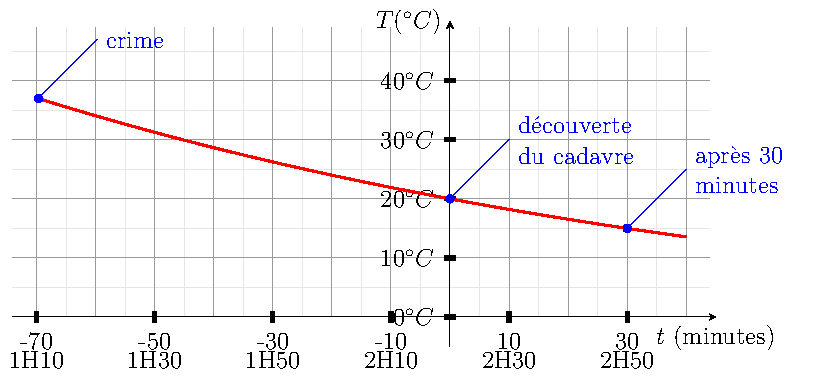
\includegraphics[width=0.65\textwidth]{solution}
\caption{Solution de l'exercice~\ref{exo.experts}}
\label{fig.solution}
\end{figure}
\end{sol}

\end{document}
